\documentclass[11pt]{article}
\usepackage{geometry}                
\geometry{letterpaper}                   

\usepackage{graphicx}
\usepackage{amssymb}
\usepackage{epstopdf}
\usepackage{natbib}
\usepackage{amssymb, amsmath}
\usepackage{hyperref}
\DeclareGraphicsRule{.tif}{png}{.png}{`convert #1 `dirname #1`/`basename #1 .tif`.png}

%\title{The Swiss Train Network}
%\author{Mario Vontobel, Elias Rieder}
%\date{date} 

\begin{document}



\thispagestyle{empty}

\begin{center}
\includegraphics[width=5cm]{ETHlogo.eps}

\bigskip


\bigskip


\bigskip


\LARGE{ 	Lecture with Computer Exercises:\\ }
\LARGE{ Modelling and Simulating Social Systems with MATLAB\\}

\bigskip

\bigskip

\small{Project Report}\\

\bigskip

\bigskip

\bigskip

\bigskip


\begin{tabular}{|c|}
\hline
\\
\textbf{\LARGE{The Swiss Train Network}}\\
\\
\hline
\end{tabular}
\bigskip

\bigskip

\bigskip

\LARGE{Mario Vontobel \& Elias Rieder}



\bigskip

\bigskip

\bigskip

\bigskip

\bigskip

\bigskip

\bigskip

\bigskip

Zurich\\
Dec 2014\\

\end{center}



\newpage

%%%%%%%%%%%%%%%%%%%%%%%%%%%%%%%%%%%%%%%%%%%%%%%%%

\newpage
\section*{Agreement for free-download}
\bigskip


\bigskip


\large We hereby agree to make our source code for this project freely available for download from the web pages of the SOMS chair. Furthermore, we assure that all source code is written by ourselves and is not violating any copyright restrictions.

\begin{center}

\bigskip


\bigskip


\begin{tabular}{@{}p{3.3cm}@{}p{6cm}@{}@{}p{6cm}@{}}
\begin{minipage}{3cm}

\end{minipage}
&
\begin{minipage}{6cm}
\vspace{2mm} \large Mario Vontobel

 \vspace{\baselineskip}

\end{minipage}
&
\begin{minipage}{6cm}

\large Elias Rieder

\end{minipage}
\end{tabular}


\end{center}
\newpage

%%%%%%%%%%%%%%%%%%%%%%%%%%%%%%%%%%%%%%%



% IMPORTANT
% you MUST include the ETH declaration of originality here; it is available for download on the course website or at http://www.ethz.ch/faculty/exams/plagiarism/index_EN; it can be printed as pdf and should be filled out in handwriting


%%%%%%%%%% Table of content %%%%%%%%%%%%%%%%%

\tableofcontents

\newpage

%%%%%%%%%%%%%%%%%%%%%%%%%%%%%%%%%%%%%%%



\section{Abstract}

This project looks at the Swiss train system. It investigates the flow of people in this transport system which is quiet important for this country. The goal was to find relations between properties like capacity, amount of people travelling, delay, fragility and more. On one hand this is approached  by a general theoretical model. On the other hand by real data. These two methods lead to a model of the Swiss train  network. On the basis of this model the properties are analysed. The Two approaches merge at end and allow us two make some statements.
 

\section{Individual contributions}

All steps are shared on github \citep{Github}
\url{https://github.com/EleSwag/Elias-und-Mario}

\section{Introduction and Motivations}

\subsection{Idea and Motivation}


Every day we travel from our homes to Zürich. The train in the morning is often very crowded and a lot of delays occur. This circumstance made us think about how the train network works and how you could handle such capacity shortages better. 
So the general idea was to model the Swiss train network and then look at its properties. This may sound like a very general question and it is and it had to be!?? As you can imagine, the whole schedule is quiet complex and consists of a lot of data. At this point we didn't know how much and what kind of data we would have access to. We heard in our lecture that the number of inhabitants has an influence on the amount of traffic. The Type of model using this approach is called Gravity model.

So we had two approaches to start with: The Gravity model, witch we will be explained in detail after, and the effort getting real data.

Because our interest in the problem came from observations in our everyday life, it was very important to us, that our work would have a strong connection to reality. To make this happen, we wrote a mail to SBB, the Swiss rail company, and asked them for real Data. Since we did not know if we would get the data we ha two make two plans.

The first possibility would have been getting a rich data set from sbb. There complex models considering the the frequency, speed and capacity of the trains and the resulting connections would be possible. In this case the question of capacity and load, and resilience were very interesting questions.

The second, alternative possibility was getting nothing. But with the gravity model we could be sure to have an angle even  without data. This was kind of a backup plan. Of course the the questions would have to be asked way more general  

So the question that draws through both approaches is:\newline 
\textbf{How do you make a good model of the Swiss train system and what statements can we make with it about the traffic flow, the capacity and the resilience of it?}    


\section{Description of the Model}
\subsection{The classical gravity model}
In  social science -especially in international economics in trade simulations- it is a common and well established approach to simulate flows with a gravity model. The motivation behind it is the physical gravity force. This is defined by $F_G:=G\frac{m_1 m_2}{r^2}$, where G is the gravity constant, $m_i$ is the mass of the  i-Th body for $i=1,2$ and r is the distance between body 1 and body 2.


This leads to the general ansatz:
\begin{align*}
F_{ij}=G\frac{M_i^{\beta_1}M_j^{\beta_2}}{D_{ij}^{\beta_3}}
\end{align*}

\citetext{\url{http://en.wikipedia.org/wiki/Gravity_model}}
We transferred this idea to our situation by identifying the mass of a city to its population and used different definitions of distance. We dropped the constant at the beginning since we normalized the resulting flow anyway. As exponents we have chosen $\beta_1=\beta_2=\beta_3=1$ since with no experience this was as suitable as anything else.\newline

\subsection{The development of the gravity model}
In our first approach we took the 10  biggest cities in regard of the number of inhabitants plus two additional ones( Olten and Arthgoldau) which are well-known important nodes of the real network.\newline
\citetext{\url{http://de.wikipedia.org/wiki/Eisenbahnknoten/\#Schweiz}}
.
We wondered if they would also become as important  in our gravity model as in the real network.\newline

To make the network more realistic we have looked up all real connections between the cities on the online train schedule (sbb.ch). Our criterion was that two nodes are connected if there exists a direct train connection between them. With this idea we didn't end with a fully-connected network which is from our point of view more realistic to simulate the direct flow between cities.

\begin{figure}
\centering
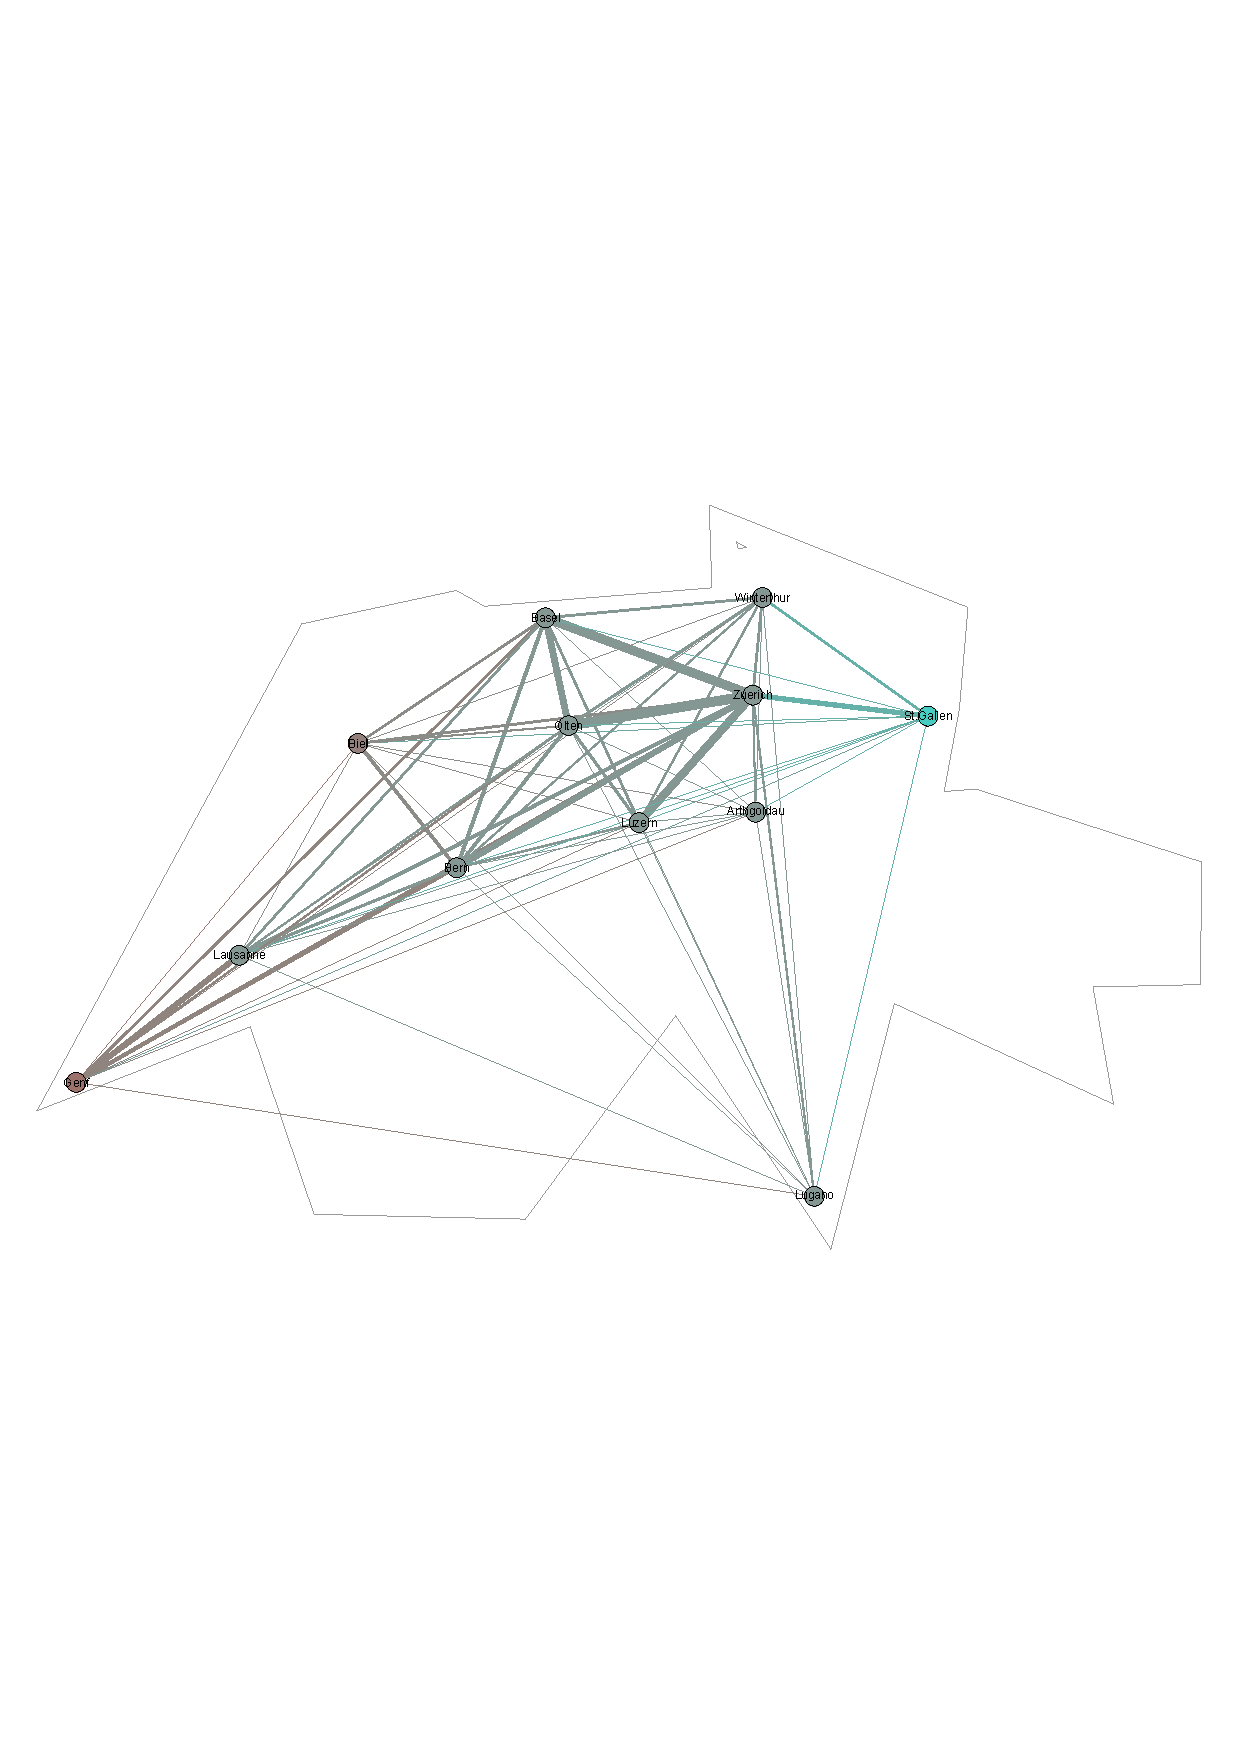
\includegraphics[scale=0.25]{switzerland_network1}
 \caption{Gravity model 1: Model of the 10 biggest cities plus two additional one. Layout by gephi with respecting geographical position.}
\end{figure}

This was the first network we plotted. While looking at the picture it was striking that the network didn't at all cover the hole country. Especially the south-west part was unattended. So we extended the number of cities to 20 and kept the two additional ones from the beginning.


\subsection{Commend on the distance in the gravity model}
In the general gravity model we used geographical distance as the distance indicator. But we thought it would also be reasonable to use the time it takes to travel from one city to the other as the distance indicator. The idea was that this also takes in account if there is obstacle like a mountain or a lake between the cities. A disadvantage of it is, that in a way one approximate the network with the existing network. Anyway we omitted that later because with the number of connection the investment grow nearly immeasurable. Also the time connection was not well-defined any more. In the sense that there were different times for the same connection.

\subsection{The Data approach}

As mentioned at the beginning the second way looking at our network was Data. Unfortunately the search for data turned out to be quiet difficult. We contacted SBB for data, but in a big company like this things are taking very long. When we finally got in contact with the right persons, there was just to less time left to process all and we could not get all the data we would have liked. Especially data about the load of the network and the capacity seems to be very sensitive. But the people from SBB were very kind and gave us what they could. They sent us a link where you public link \citetext{\url{http://gtfs.geops.ch}} were you can download the whole timetable in Gtfs-Format (General Transit Feed Spesification). Sadly we could not involve that, because of the already mentioned time shortness. We also could sent several questions to one of their networkspecialists.(Anhang:index x y z.....). Especially the numbers of people boarding and de-boarding for a few big cities made us curious. This is a number we maybe could relate with our gravity models.  


\section{Implementation}
\textbf{In general we tried to be as specific as possible with the annotation of the functions in matlab}

We created a script called data1 which contains all our relevant data.

\subsection{Network flow-function}
First we implemented a general network function which apply the theory mentioned in the description of the model to an adjacency matrix of a network. This function gave another adjacency matrix back with the simulate flow. This function would also run for every other gravity model based simulation.\newline

For the distance based gravity function we also need the geographical distance. For that purpose we added to each city its coordinates and computed the distance between each city by just applying Pythagoras. Since Switzerland is a small country we did not taken in account that the earth is a sphere and just approximated as if it was a plane. The function gives again a adjacency matrix back.


\subsection{Visualization}
In the lectures it was recommended to use gephi. So some of our pictures are made with it. But a huge disadvantage of gephi is that it is rather complicated to respect geographical position if one uses an adjacency  matrix to represent the network. In figure 1 we placed the cities by hand.

But since this is rather complicated we also wrote function in matlab to illustrate a network given in a adjacency matrix. The result isn't as pretty as in gephi so both methods have their advantages and disadvantages.


\begin{figure}
\centering
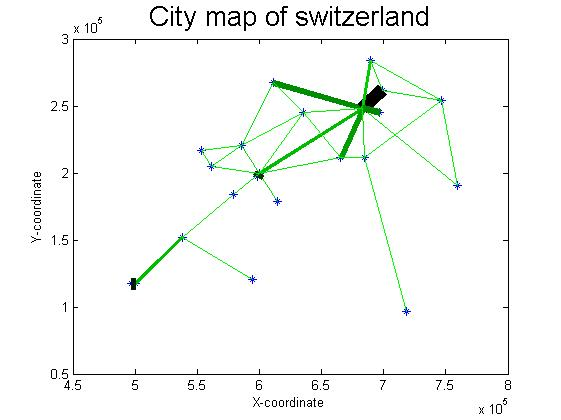
\includegraphics[scale=0.5]{switzerland_network2}
 \caption{Gravity model 2: Model of the 20 biggest cities plus two additional one. Layout by matlab. The strength of a connection is emphasized by the thickness as well as the depth of the colour from the line.}
\end{figure}

\subsection{Investigation-function}
To investigate the network we strongly relaid on the paper 'Complexity in human transportation networks: a comparative analysis of worldwide air transportation and global cargo-ship movements'.
We implemented the shortest distance function described on page 592/593. At the beginning we had a hard time to find the right function but then Mario remembered that he had in the fall semester 2013 a lecture on algorithm and complexity. Mostly the lecture was about theory from trees (special case of a graph) but there was also a part on general graph theory. In that part was the 'Floyd-Warshall'-algorithm which does exactly what we needed. Which means shortest paths between all nodes.
The notes also allowed as to implement a function which checks if a network is still connected by using a 'depth-first-search'-algorithm.




\section{Simulation Results and Discussion}

\subsection{General Network Parameters}
\begin{tabular}{c|c|c|c|c|c|c|c|c|c|}
 & N & L & $\sigma$ & $\phi$ & $d_T$ & $\langle r\rangle$ & 
 $\langle w\rangle$ & $\langle F\rangle$&$\langle k\rangle$ \\\hline
 Full-connected & 22 & 231 &0.9545&1& 0.8413& $2.6604e+07$&0.0275&0.5781& 21\\\hline
 
 Other & 22 & 34 &    0.1405&2.9134& 11.0154&$2.6028e+07$&0.1037&0.3215& 3.1364\\\hline
\end{tabular}


\subsection{Networkflow}

To determine how powerful the gravity model is, you have to be very careful about your question. It strongly depends of your point of view. If you want to get a impression of the amount of traffic of the 10 biggest cities in Switzerland (ev results korrelation fo), you might get quiet good results. But if you slightly change your point of view and ask yourself in which cities of Switzerland a big amount of traffic occurs, your gravity model might not be overall correct. Best example is Olten. Small number of inhabitants big amount of traffic. Even one of the seat critical trains (train were you might have to stand) (reference), departs from olten

The other, pretty obvious weakness of the gravity model are time variable flows. Of course you cant. We learned that taht this a quiet important aspect  if you want to find out something about capacity of this network. The fastest growing traffic flows in the network are the peaks in the rush-hour. (Geschäftsberich s 07)

\subsubsection{Comparison of our flow with the real flow from some nodes}
fullconnected network:$\begin{bmatrix}
    1.4788\\
    0.4861\\
    1.0764\\
    1.3305\\
    0.8769\\
    0.8358\\
    1.2380\\
    0.9914\\
         0\\
    0.9778\\
         0\\
         0\\
         0\\
         0\\
         0\\
         0\\
         0\\
         0\\
         0\\
         0\\
    6.6792\\
         0
\end{bmatrix}$
connected network:$\begin{bmatrix}
    0.2048\\
    0.0825\\
    0.2865\\
    0.4284\\
    0.1246\\
    0.1264\\
    0.2470\\
    0.4781\\
         0\\
    0.2264\\
         0\\
         0\\
         0\\
         0\\
         0\\
         0\\
         0\\
         0\\
         0\\
         0\\
    1.0052\\
         0

\end{bmatrix}$

\begin{figure}
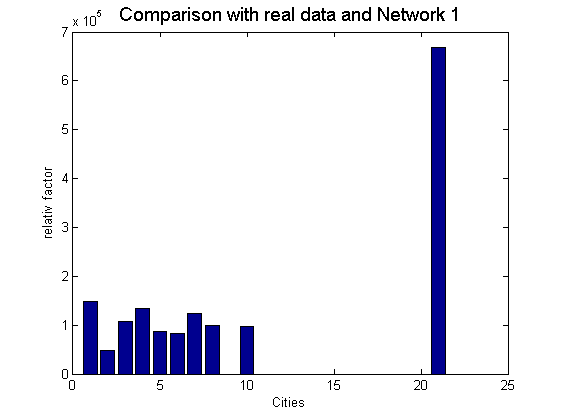
\includegraphics[scale=0.5]{compare1}
 \caption{resonalbe description}
\end{figure}

\begin{figure}
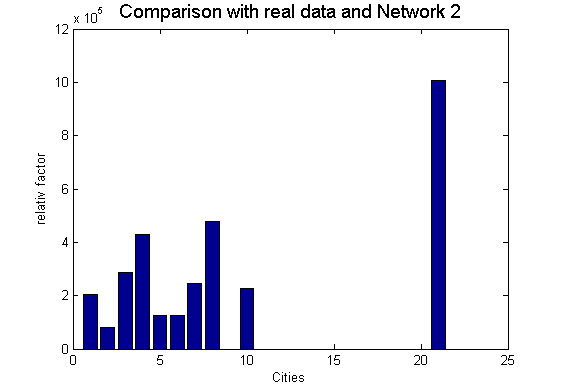
\includegraphics[scale=0.5]{compare2}
 \caption{resonalbe description}
\end{figure}



\subsection{Resilience}
 Resilience breaks down to a combinatoric problem. Some trivial solutions (Lugano)
 
 sbb assured us they have replacement train at important nodes:D

....

\subsection{capacity}

Unfortunatley none of our approaches could answer our qwestions about capacity. The Gravity model can give Information about the amount of traffic, but it doesn't tells anithing about how big this flows can get. What SBB told us is, how they deal with it "If the route allows it, the train is maid as long as possible. All Platforms where the train stops have to be long enough. As additional action additional trains are added during the rush our"..."Alternatively the rolling stock can be optimised. On routes with little space, rolling stock with high capacity is used. If all these actions don't suffice, an extension is required" (Reference zu Questions). One other thing they mentioned is, that their trying to foster flexible worktime and homeoffices. Their doing this by negotiating with other big employers. (reference mail mueller 3. dez, + article in mail). This all seems all to be aimed at decresing the rushour peaks.  




\section{Summary and Outlook}

Outlook:
We found out quiet interesting things about the Swiss train network. Of course it would have been nice if we could have found more answers but we found some interesting trails who would be worth investigating further
The rushour peaks: 


\section{References}

\bibliography{reference}


\end{document}  